\documentclass[tikz,border=3mm]{standalone}
\usetikzlibrary{arrows.meta, positioning}

\begin{document}
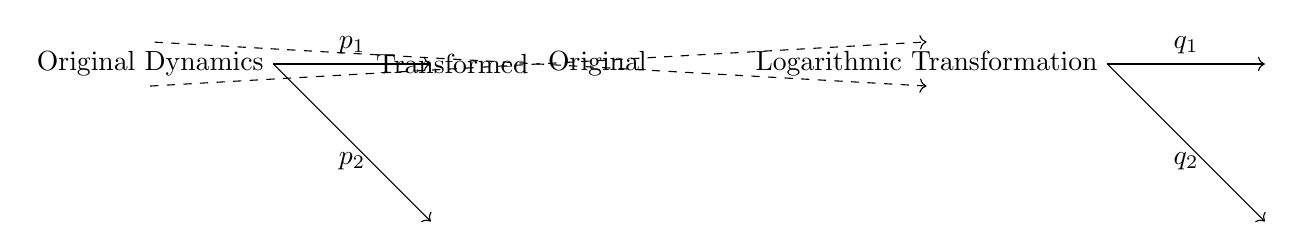
\begin{tikzpicture}[node distance=2cm]
    % Left side: Original Dyson-Schmidt dynamics
    \node (left_dynamics) {Original Dynamics};
    \draw[->] (left_dynamics.east) -- node[above] {$p_1$} ++(2,0);
    \draw[->] (left_dynamics.east) -- node[below] {$p_2$} ++(2,-2);
    
    % Right side: Logarithmic transformation
    \node[right=of left_dynamics, xshift=4cm] (right_transform) {Logarithmic Transformation};
    \draw[->] (right_transform.east) -- node[above] {$q_1$} ++(2,0);
    \draw[->] (right_transform.east) -- node[below] {$q_2$} ++(2,-2);
    
    % Arrows between the two sides
    \draw[dashed, ->] (left_dynamics.south) -- node[left] {Transformed} (right_transform.north);
    \draw[dashed, <-] (right_transform.south) -- node[right] {Original} (left_dynamics.north);
\end{tikzpicture}
\end{document}